\chapter{The Bethe-Peierls solution}

The Bethe-Peierls solution was the first attempt to solve the BLSG model. Using the fact that the factorization approximation is exact on tree-like structures, the solution finds a self consistent equation for the field distribution $Q(h)$. However, we will se that the BP solution is not valid in the region of the glassy phase (under the critical temperature).In the low temperature phase we have to perform a much more refined computation (and we will do it in the following chapter).
In the next part of this chapter, the BP solution will be also referred as the replica symmetric (RS) solution. In fact, we will prove in the last section that the BP solution is equivalent to a replica symmetric solution in the replica framework \cite{bethe}.
A good description of the Bethe Peierls approximation in more general terms is available at \cite{montanari}.
The states structure at zero temperature, the phase transitions diagram and an algorithm generated for finding the ground states are discussed in \cite{tersenghi}.

Using the fact that no closed loops are present it is possible to solve
the problem by iteration \cite{hans}.
Our first task will be to write the partition function on a given site $\sigma_0$, which can be written formally as
a function of the local fields acting on $\sigma_0$

\begin{equation}
Z = \sum_{\sigma_0,\sigma_1,\ldot,\sigma_k} \exp{\beta( \sigma_0 \sum_{i=1}^{K} J_i \sigma_i + \sum_{i=1}^{K}h_i \sigma_i )}
\label{partition}
\end{equation}

Using the fact that $\sigma_0$ can only take values ${\pm1}$ it is possible to write each term of the partition function explicitly summing over $\sigma_0$

\begin{equation}
\sum_{ \sigma} \exp{ \beta ( \sigma_0 J \sigma + h \sigma)} = c(J,h)\exp{\beta u(J,h) \sigma_0}
\label{u}
\end{equation}

Where the two auxiliary function are defined as

\begin{equation}
u(J,h) = T \tanh^{-1}[\tanh(\beta J)\tanh(\beta h)]
\end{equation}

\begin{equation}
c(J,h) = 2 \frac{\cosh(\beta J)\cosh(\beta h)}{\cosh(\beta u(J,h))}
\end{equation}

We will see that the function $u(J,h)$ will return often in this discussion.
If we look the new form of equation \ref{u} we can see that in the new framework the effective Hamiltonian acting on $\sigma_0$ is the sum of the variables $u_1,\dots,u_K$ of each neighbor. We will call local field each $h_j$ interacting with a considered site.

If we sum the contribution from each branch, we can write
the magnetization on $\sigma_0$

\begin{equation}
\langle\sigma_0\rangle = \tanh(\beta h_0)
\label{sigma0}
\end{equation}

where $h_0$ is simply given by the sum of each effective field acting on $\sigma_0$.

\begin{equation}
h_0 = \sum_{i=1}^K u(J_i,h_i)
\label{merge}
\end{equation}

\begin{figure}
	\centering
		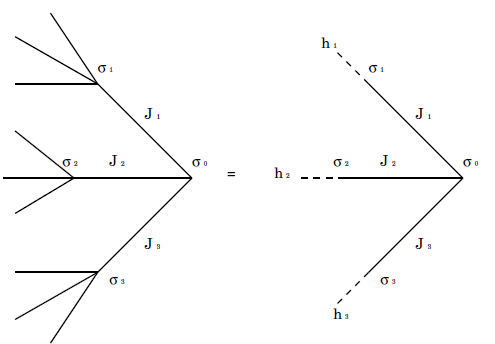
\includegraphics{img/tree.png}
	\caption{Pictorial representation of local fields on their branches}
	\label{fig:tree}
\end{figure}



\section{Cavity method for the Bethe lattice}

Before going on it is useful to recall the basic operations that will be used frequently in the elaboration. The formalism used in the next sections is usually referred as cavity method (\cite{beyond} for some generalities on the cavity approach). Since a large number of papers has been written on cavity method, here I will only remark the main tool we are going to use most frequently, that is the iteration procedure. We will show the method applied to the Cayley tree, since our utilization of it is directly aimed at a solution of the Bethe lattice spin glass.
Suppose to remove a random site from a Cayley tree(among with each of the links connected to it), now the system is divided into a number of subsystems equal to the coordination number $K+1$. Each subsystem is locally identical to the starting one.
Now suppose to have $K$ of these subsystems; if we pick up the root of each of those and merge into the site 0, we obtain an object that can be used to be merged to generate a bigger system, where now the site 0 is the root of one of the $K$ branches.

\begin{figure}[h]
\centering
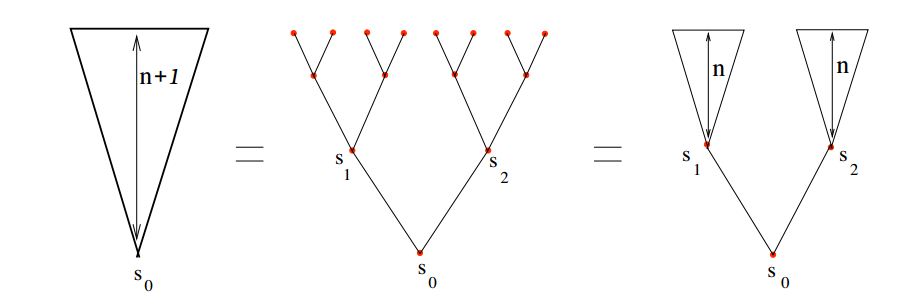
\includegraphics[scale =0.6]{img/cavity.png}
\caption{Scheme of the iteration procedure}
\label{fig:cav}
\end{figure}

This framework gives a method to obtain a recursion relation useful to solve the problem (that will be derived in the next lines) and an operative way to evaluate the relevant thermodynamic observables.
By imposing that each $u_j$ is derived from the same probability distribution $Q(h_j)$ of the site 0 we obtain a self consistent equation for $Q(h)$

\begin{equation}
Q(h) = \int dh_1Q(h_1),\ldots,dh_KQ(h_K) \delta(h-h_0)
\label{RS}
\end{equation}

In order to find the distribution of equilibrium local fields , given the distribution on a branch, we have to do the same operations as before, but now merging $K+1$ branches into one site. In this way we are adding a site fully connected to his neighbors, which cannot be used for an iterative costruction of the Bethe lattice, but will be used to find the site dependence of any relevant observable. When we add a site connected to $K+1$ branches we have

\begin{equation}
Q_t(H) = \int dh_1Q(h_1),\ldots,dh_KQ(h_K+1) \delta(h-H_0)
\label{true}
\end{equation}

\begin{figure}[h]
\centering
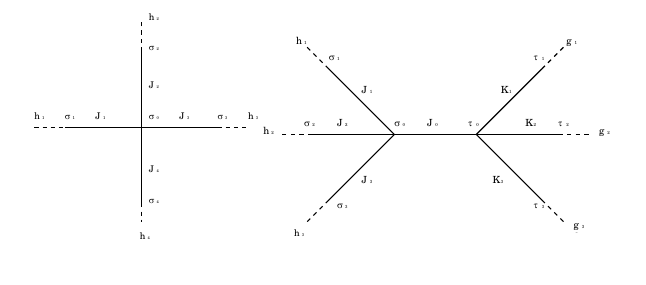
\includegraphics[scale =0.8]{img/sitebond.png}
\caption{Site and link contributions, in this figure the bonds linking the $\tau$ spin are labeled as $K_i$ (not to be confused with the coordination number K).}
\label{fig:sitebond}
\end{figure}

The field $H_0$ is calculated similarly to eq. \ref{merge} but this time using $K+1$ branches.

It is also possible to add a new link to the system, this time using a cavity link and, as a consequence, two cavity spins. Let's call these two spins $\sigma$ and $\tau$. These spins will be connected to $K$ neighbors, and when we add the new link $J_c$, they will be each other's $K+1$th neighbor.

Adding a link allows us to obtain the energy of the model (we remember that the energy $E$ is given by $E = \langle \mathcal{H} \rangle$). Since the Hamiltonian of the model is given by \ref{hamiltionian} the energy of the new link is simply given by

\begin{equation}
E_{c} = - J_c \langle \sigma \tau \rangle_c
\label{ec}
\end{equation}

where the average has a Gibbs measure with an effective Hamiltonian $\mathcal{H}_c$ which is given by

\begin{equation}
\mathcal{H}_c = - J_c \sigma \tau + h_0(\sigma)\sigma + h_0(\tau)\tau
\label{hc}
\end{equation}

where $h_0(\sigma)$ is the local field acting on $\sigma$ (given by $\tau$) before the insertion of the cavity link.
Using equation \ref{hc} in equation \ref{ec} allows us to find $E_c$: a simple computation gives a value for $E_c$ given by

 \begin{equation}
{E}_c = - J_c \frac{\tanh(\beta J_c)+\tanh(\beta h_0(\sigma))\tanh(\beta h_0(\tau))}
{1+\tanh(\beta J_c)\tanh(\beta h_0(\sigma))\tanh(\beta h_0(\tau))}
\label{links}
\end{equation}

\section{Overlaps and free energy evaluation}

The first observable we are going to evaluate, as a simple example, is the Edwards Anderson order parameter,$q ={1\over N} \sum_i \langle\sigma_i\rangle^2$.
Using \ref{sigma0} we can write $q$ as a weighted sum over the values of $H$

\begin{equation}
q = \int dHQ(H) \tanh(\beta H)\tanh(\beta H)
\label{qsite}
\end{equation}

It is also possible to compute the link overlap, which can be deduced from the iterative fields distribution, $Q(h)$ as ($E_J$ is the average over the $J$ distribution):

\begin{equation}
q_l = E_J \int dh_1Q(h_1)dh_2Q(h_2) \frac{\tanh(\beta J)+\tanh(\beta h_1)\tanh(\beta h_2)}
{1+\tanh(\beta J)\tanh(\beta h_1)\tanh(\beta h_2)}
\label{qlink}
\end{equation}


The free energy in this solution is evaluated as follows (for improved references one may see \cite{bethe} and \cite{katsu}):
First one must evaluate the site contribution to the free energy on the site $i$, then sum over the values of $\sigma_i$.

\begin{equation}
\beta {F_s}_i = \ln \sum_{\sigma_i} \exp(-\beta H_i \sigma_i )
\label{siteF}
\end{equation}

The link contribution is slightly more involved, as we need to add a cavity link, together with two cavity spins.
After a little computation and using equation \ref{links} is possible to write the link contribution to the free energy (\cite{bethe})

\begin{equation}
\beta {F_l}_ij = \ln \sum_{\sigma_i} \exp(-\beta H_iH_j \sigma_i\sigma_j )
\label{linkF}
\end{equation}

When both contributions have been obtained, it becomes possible to write the total free energy as the sum of the two contributions.
\begin{equation}
F = {K+1 \over 2}\sum_i F_l -KF_s
\label{RSF}
\end{equation}



\section{Computer implementation of the solution}

In order to control the correctness of the just proposed solution, it is possible to implement the solution just described using a population dynamics algorithm. This method has previously
been used in \cite{bethe} for the BLSG, and in \cite{self}

The algorithm is composed of a few little steps.

\begin{enumerate}
    \item{Generate $N_h$ fields. Fields may be i.i.d. random variables in the unitary interval, as example.}
    \item{Choose $K$ sites at random, among with $K$ values for $J$.}
    \item{Generate the field $h_0$ using \ref{merge}.}
    \item{Choose a site $i$ to update, this can be either random chosen or sequentially chosen.}
    \item{Substitute $h_i$ with $h_0$. Start again from point 2.}
\end{enumerate}

In this way one generates a Markov process in the fields distributions.
After a sufficient number of iterations is performed, the fields distribution will converge to the equilibrium one. We will see that, due to the presence of RSB in the low temperature phase (which has as a consequence a non ergodic behaviour of the system) this convergence is not assured, and the algorithm will need some improvements.

While this procedure generates the correct field distribution, it shall not be used to evaluate the site and field observables. In order to evaluate the overlaps, the internal energy and the free energy, we have to do the same operation as before, this time adding a new site to the system and a new link. Thus we have to merge $K+1$ branches into a new site for the site contributions, and we have to insert two new spins attached to $K$ branches each, and then merge those two, in order to get the correct link distribution. Once obtained these two one can evaluate every observable using equations \ref{qsite}, \ref{qlink}, \ref{siteF} and \ref{linkF}.

\subsection{Where the solution works}

If we solve numerically eq.\ref{RS} we note that, at least in the high temperature regime, we  have a paramagnetic solution. Surely if we put $Q(h) = \delta(h)$  \ref{RS} is satisfied. The solution is thus stable at high enough temperatures.
This was easily predictable: at high enough temperatures it is well known that finite connectivity spin glasses behave as paramagnets.

If we look at a numerical solution of equation \ref{RS} we may note that in the low temperature phase the $\delta$ solution becomes unstable. Past studies have shown that an evaluation of specific heat and entropy leads to a negative value for inverse temperatures $\beta>\beta_c$, where $\beta_c$ is given by the relation
\begin{equation}
\< \tanh( \beta_c J )\>_J = 1/K
\end{equation}



The instability of this solution has been widely investigated \cite{instability},\cite{thou},  \cite{tersenghi}. If considering the lattice used in my simulations and in \cite{zullo}, $K = 6$ and the inverse critical temperature is near 2.3.
The authors of \cite{zullo} performed simulation at temperature $T=0.8$, widely under the critical temperature.
In order to compare the results of the RS algorithm with the ones found in literature, the algorithm will run with $K=6$ and $T=0.8$.
The values returned by RS algorithm are reported in the following:

\begin{equation}
F = -1.863 \pm 0.001 \hspace{1 cm},U = -1.816 \pm 0.001 \hspace{1 cm}, q_0 = 0.683 \pm 0.001
\end{equation}

As we can see, the value of the internal energy $U$ totally disagrees with the one found in simulations.

\begin{figure}
\centering
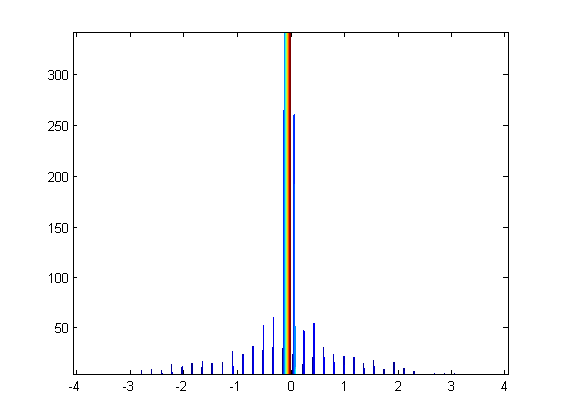
\includegraphics[scale 0.7]{img/fieldvsbeta.png}
\caption{The low temperature distributions (in blue) are not a \delta(h)}
\label{fig:}
\end{figure}


\section{Replica approach to the problem}

We ofter referred to the Bethe Peierls calling it the replica symmetric solution. In fact it is possible to prove the equivalence between the Bethe Peierls solution and a replica symmetric approximated solution in the replica framework. Details on the replica approach to spin glasses are available in all the major literature (examples are \cite{beyond} \cite{glass}). A computation of the free energy $F$ with the replica approach has been performed in \cite{replica}. In this paragraph we will only show that the replica symmetric free energy is equal to the one found in eq.\ref{RSF}.

In the replica framework the partition function \ref{partition} is replicated $n$ times. This means that now $\sigma$ in a n-dimensional vector of Ising variables. In order to reproduce the correct result, $n$ must go to zero at the end of the computations. In \ref{partition} the authors introduce a replica probability distribution, $\rho(\sigma)$ and the free energy functional $ F_r[\rho(\sigma)]$ with a structure similar to the variational free energy proposed in \ref{bethe}.
Let us report only the final result of the computation. Calling $f_r$ the free energy density $ F_r[\rho(\sigma)]/N$ we have

\begin{equation}
-\beta n f_r = {k+1\over2}\ln(\Tr_{\sigma,\tau} \rho(\sigma)^K\rho(\tau)^K \exp\sum_i \beta J \sigma_i \tau_i) -
k \ln Tr_\sigma \rho(\sigma)^{K+1})
\end{equation}

Let us comment this equation. As we can see, the free energy density is composed of two terms. The first is the same link contribution obtained in the previous section, while the other is exactly the site contribution. The link contribution has a K-th power because while we connect two cavity spins, each of those must be connected to $K$ sites, in order to maintain the fixed connectivity. On the contrary, the site contribution contains a power $K+1$.

If we set ${\delta F \over \delta \rho} = 0$ we obtain then correct replica free energy.

\section{Free energy shift}

It is possible to compute the mean free energy in the cavity approach, computing the free energy shift $\Delta F$ obtained by adding a new site or a new link to the system. The reason behind this equivalence can be explained as follows \cite{enzo}: when the equilibrium phase is reached, the total free energy may be written as $F_N = fN$; when adding a new spin we can simply write $F_{N+1} = f(N+1)$ and thus obtain the free energy per site by simply having $f = F_{N+1} - F_N \equiv \Delta F$.

Let's start by computing the site contribution to the free energy shift, $\Delta F_s $. Using the equation \ref{partition} and knowing that $\mathcal{Z} = \exp{-\beta F)$ we may write (\cite{bethe})
\begin{equation}
\beta \Delta F_s = \ln[2\cosh(\beta\sum_{i}^{K+1} u(J_i,h_i))] + \sum_{i}^{K+1} \ln[{\cosh\beta J_i \over \cosh \beta  u(J_i,h_i)}]
\label{sitedf}
\end{equation}

The bond contribution is more complicated, since it must be averaged over the $\sigma$ $\tau$ distribution.
\begin{eqnarray}
\beta \Delta F_l &=& \sum_{i}^K+1 \ln { \cosh (\beta J_i) \cosh (\beta L_i) \over  \cosh(beta u(J_i,h_i))\cosh(beta u(L_i,g_i))} \nonumber \\
&+&\ln[ \sum_{\sigma,\tau}\exp( \beta J \sigma \tau + \beta\sigma \sum_i^K u(J_i,h_i) \beta\tau\sum_i^K u(L_i,g_i) ) ] \nonumber \\
\label{linkdf}
\end{eqnarray}
In the above equation the variables $g_i$ represent the local fields acting on $\tau$, and $L_i$ are the bonds between each site.
The mean free energy is then evaluated as the sum of each site and bond contribution:
\begin{equation}
F = {(K+1)\over 2}\delta F_l - K \delta F_s
\end{equation}

It is also useful to report the iterative free energy shift, that is the free energy shift obtained when adding a site in the iterative construction of the Bethe lattice. It is simply given by the site contribution just evaluated, this time merging $K$ branches instead of $K+1$:
\begin{equation}
\beta \Delta F_{iter} = \ln[2\cosh(\beta\sum_{i}^K u(J_i,h_i))] + \sum_{i}^K \ln[{\cosh\beta J_i \over \cosh \beta  u(J_i,h_i)}]
\label{iterdf}
\end{equation}
This free energy shift will turn useful in the next chapter, when we will compute the probability distribution $Q(h)$ in the one step RSB framework. 